\documentclass[a4paper]{article}

\usepackage{fullpage}
\usepackage{listings}
\usepackage{url}
\usepackage{forest}
\usepackage{graphicx}

\definecolor{folderbg}{RGB}{124,166,198}
\definecolor{folderborder}{RGB}{110,144,169}

\def\Size{4pt}
\tikzset{
  folder/.pic={
    \filldraw[draw=folderborder,top color=folderbg!50,bottom color=folderbg]
      (-1.05*\Size,0.2\Size+5pt) rectangle ++(.75*\Size,-0.2\Size-5pt);  
    \filldraw[draw=folderborder,top color=folderbg!50,bottom color=folderbg]
      (-1.15*\Size,-\Size) rectangle (1.15*\Size,\Size);
  }
}

\begin{document}

\title{\Huge\bfseries Robot Simulator, v160505}
\date{5th May, 2016}

\maketitle

\section*{A Word of Caution}

Simulators, by their very nature, are approximations of the real world. Various short cuts are made to implement them and, as a result they do not model the world perfectly. Therefore, they should be treated as an {\itshape aid\/} to the development of your system. It does not replace use with the actual robotic platforms.

\section*{Version History}

\begin{itemize}
\item {\bfseries 160430}: Initial release
\item {\bfseries 160505}: Include methods for custom setting of encoder ticks.
\end{itemize}

\section*{Prerequisites}

The simulator has been tested to work on Ubuntu Linux 15.10, Mac OSX 10.11.4 and Windows 10, 64-bit edition. It uses standard software with no third party dependencies, and is likely to work on other platforms with minimal changes.

To run the simulator, you will need:

\begin{itemize}
\item Java JRE 1.7 or above, \url{https://java.com/en/download/}
\item A C++11 (or above) compliant compiler, including gcc, clang, or Visual Studio.
\item CMake, version 3.1.0 or above, \url{https://cmake.org/download/}.
\end{itemize}

\section*{Package Structure}

Uncompress the zip file, gives the following directory structure:

\begin{forest}
  for tree={
    font=\ttfamily,
    grow'=0,
    child anchor=west,
    parent anchor=south,
    anchor=west,
    calign=first,
    inner xsep=7pt,
    edge path={
      \noexpand\path [draw, \forestoption{edge}]
      (!u.south west) +(7.5pt,0) |- (.child anchor) pic {folder} \forestoption{edge label};
    },
    before typesetting nodes={
      if n=1
        {insert before={[,phantom]}}
        {}
    },
    fit=band,
    before computing xy={l=15pt},
  }  
[robotsimulator
  [Client
    [applications
    ]
    [Examples
    ]
    [include
    ]
    [src
    ]
    [tests
    ]
  ]
  [Documentation
  ]
  [Simulator
  [bin
  ]
  [lib
  ]
  [maps
  ]
  [src
  ]
]
]
\end{forest}

\subsection*{Simulator}

This was built using Java in Eclipse. The Eclipse project is included, but a precompiled, runnable jar file (\verb+Simulator/bin/simulator.jar+) has also been included and this can be run directly. You might need to give it permission to act as a server in a firewall.

\subsection*{Client}

Unlike the server, the client is in C / C++ code and must be built on the local operating system / build environment. The client consists of a library, \verb+libclient+, which includes a networking library (\verb+Client/src/Practical_Socket+), a library for linking with the simulation (\verb+Client/src/Client+) and a port of a number of the standard Propeller IDE libraries (in \verb+Client/src/Simple_Libraries+).

The meta-build system \verb+cmake+ (\url{https://cmake.org/}) is used. \verb+cmake+ uses high-level text files to specify a project. It can use these to generate build systems for a huge range of development platforms (including makefiles, Visual Studio solutions, nmake makefiles, Xcode projects, and eclipse workspaces) for a huge range of platforms (including OSX, Linux, Windows, and Cygwin under Windows).

On a linux, OSX or Cygwin, the easiest approach is to run it directly from the command line. No additional configuration is required. The command is:

\begin{verbatim}
Hnatt:Client ucacsjj$ cmake .
-- Looking for pthread.h
-- Looking for pthread.h - found
-- Looking for pthread_create
-- Looking for pthread_create - found
-- Found Threads: TRUE  
-- Configuring done
-- Generating done
-- Build files have been written to: /Users/ucacsjj/Proj/Simulator/Code/Trunk/Source/Client
\end{verbatim}

The code can then be built using:

\begin{verbatim}
Hnatt:Client ucacsjj$ make
[  1%] Building CXX object src/CMakeFiles/client.dir/Practical_Socket/PracticalSocket.cpp.o
[  1%] Building CXX object src/CMakeFiles/client.dir/Client/Console.cpp.o
[  1%] Building CXX object src/CMakeFiles/client.dir/Client/ServerConnection.cpp.o
[  2%] Building CXX object src/CMakeFiles/client.dir/Client/launcher.cpp.o
[  2%] Building CXX object src/CMakeFiles/client.dir/Client/simulator.cpp.o
[  3%] Building CXX object src/CMakeFiles/client.dir/Simple_Libraries/Motor/libservo/servo.cpp.o
[  3%] Building CXX object src/CMakeFiles/client.dir/Simple_Libraries/PropellerGCC/cog.cpp.o
[  4%] Building CXX object src/CMakeFiles/client.dir/Simple_Libraries/PropellerGCC/CogManager.cpp.o

....

[100%] Linking CXX executable Cog_Info_Exchange
[100%] Built target Cog_Info_Exchange
[100%] Building C object applications/CMakeFiles/spinLeftRight.dir/spinLeftRight.c.o
[100%] Linking CXX executable spinLeftRight

\end{verbatim}

You may see a number of warnings. These can be ignored in the library here.

For Windows, the easiest approach is to use the \verb+cmake+ GUI. Instructions on its use can be found at \url{https://cmake.org/runningcmake/}. It requires no special configuration.

\section*{Usage}

\subsection*{Simulator}

For the simulator, simply double click on the jar file to open. This should present you with the window:

\begin{center}
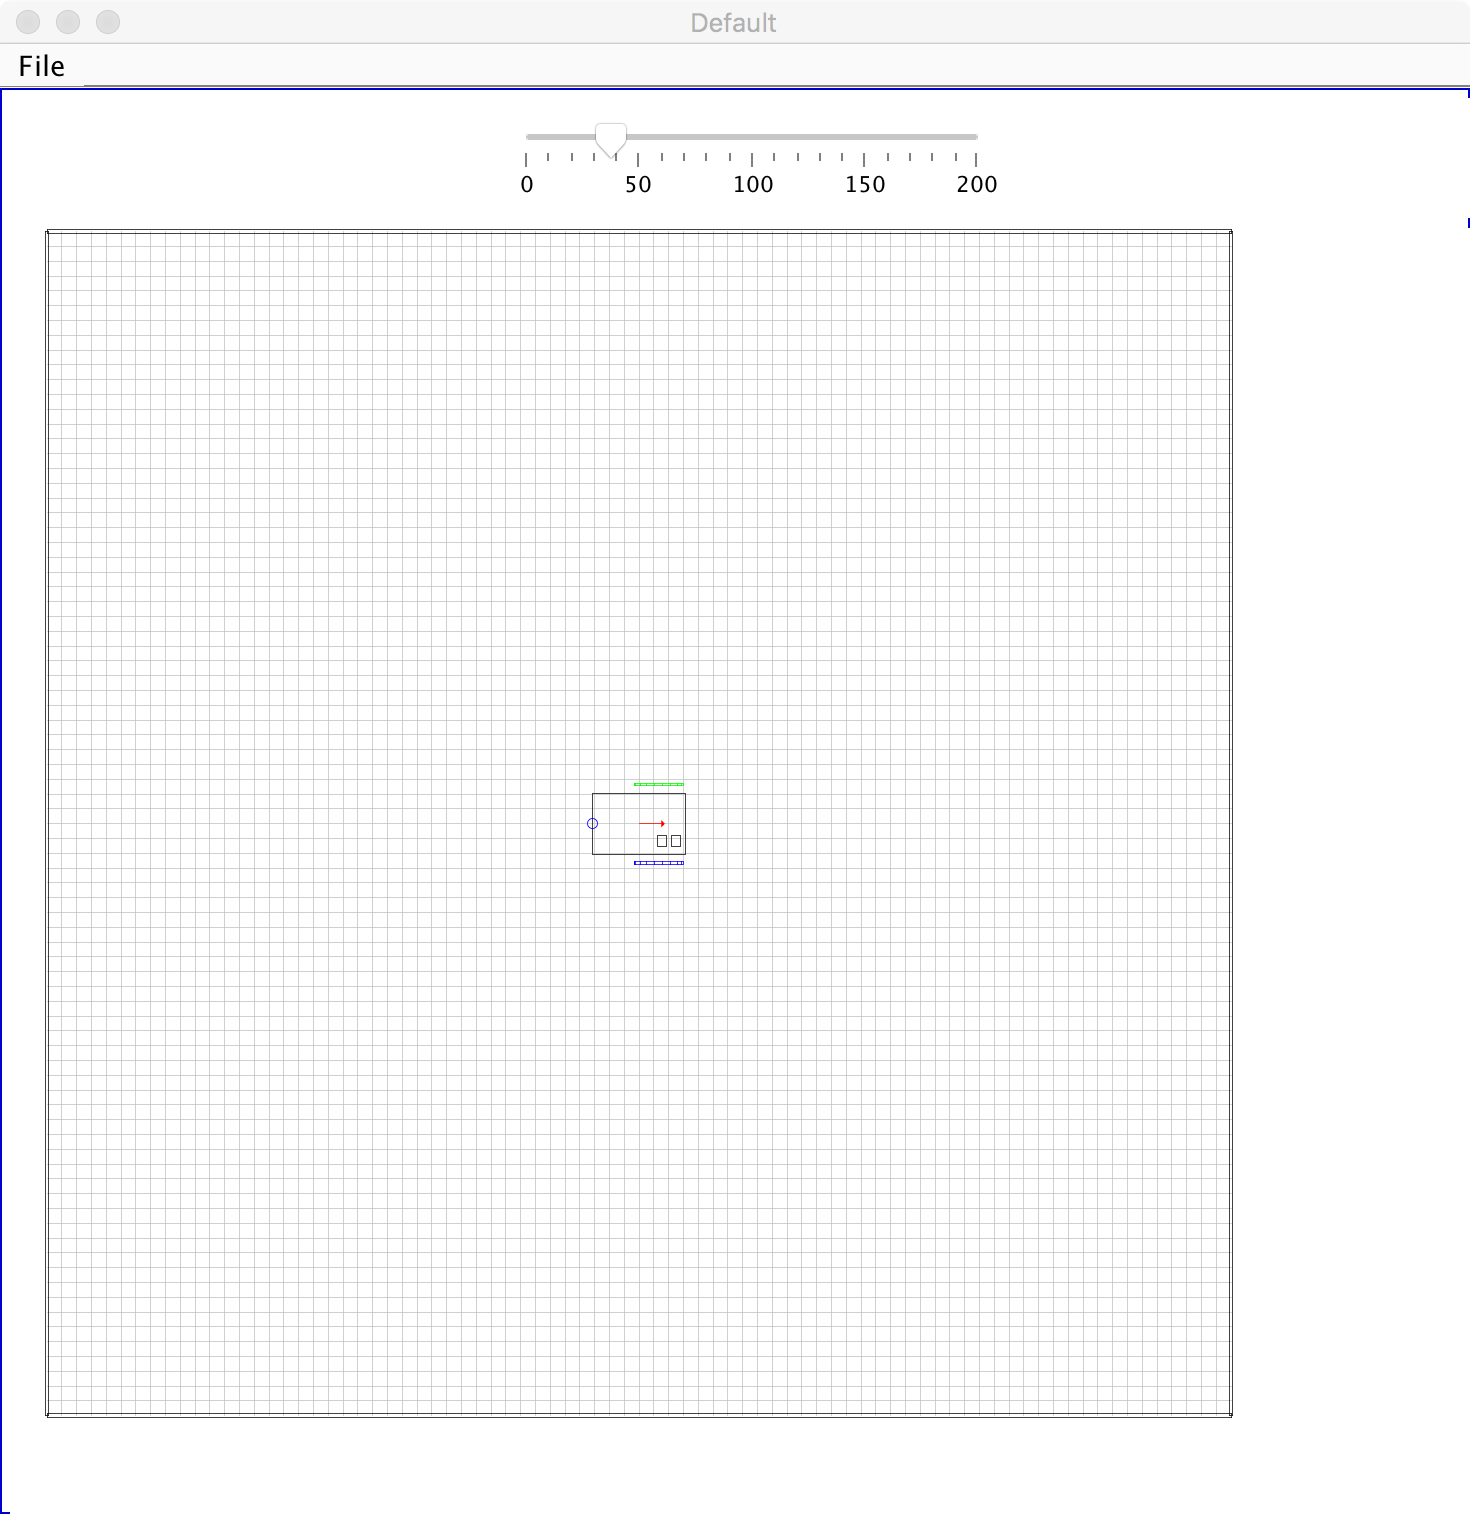
\includegraphics[width=0.5\linewidth]{default_scenario.png}
\end{center}

The GUI options are (deliberately) very simple. The slider only changes the zoom setting (the mousewheel or equivalent can be used to zoom in and out).

The \verb+File+ menu supports loading a map from file, refreshing a map (which reloads a previous specified map) or exiting.

The maps are all in the \verb+Simulator/maps+ directory. The figure below shows the map obtained from loading Maze 02:

\begin{center}
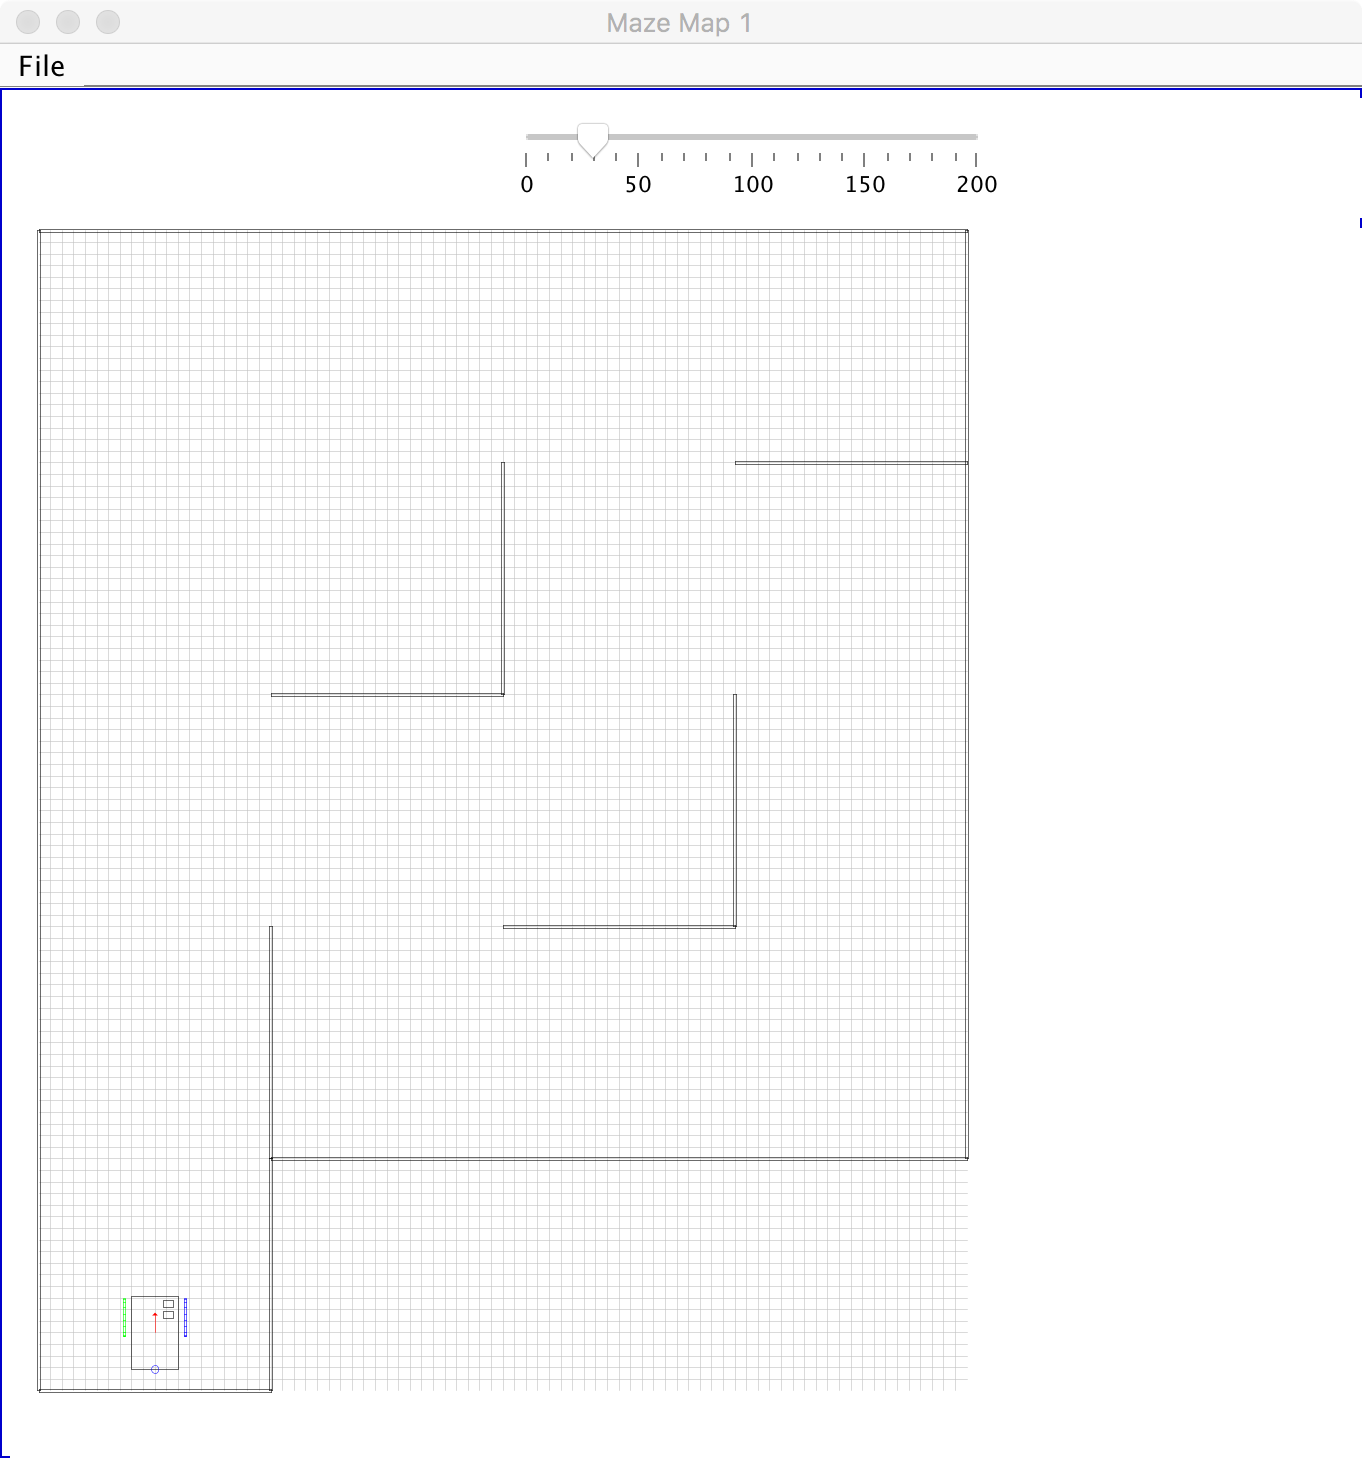
\includegraphics[width=0.5\linewidth]{Maze_Map01.png}
\end{center}

\subsection*{Client}

Any program you build will be linked into a command line application. You should be able to build most applications ``out of the box'' without any modification. (The only requirement is that \verb+simpletools.h+ \emph{must\/} be included by the file which includes the declaration of the \verb+main+ function.)

For example, consider the contents of \verb+Client/tests/testDriveSpeed.c+:

\lstset{language=C++} 

\begin{verbatim}
#include <stdio.h>
#include <stdlib.h>
#include <time.h>

#include "abdrive.h"
#include "simpletext.h"
#include "simpletools.h"
#include "ping.h"

int main(int argc, const char* argv[])
{
  // Drive ahead nice and slow
  drive_speed(16, 16);

  struct timeval tv;
  
  gettimeofday(&tv, NULL);

  long int startSecs = tv.tv_sec;
  
  while(ping_cm(8) > 8)
    {
      pause(100);
      struct timeval now;
      gettimeofday(&now, NULL);
      if (now.tv_sec != tv.tv_sec)
        {
          int left, right;
          drive_getTicks(&left, &right);
          printf("%ld %d %d\n", now.tv_sec-startSecs, left, right);
          tv.tv_sec = now.tv_sec;
        }
    }
}
\end{verbatim}

This program sets up the drive speed so that the robot slowly trundles forwards and, once per second, prints out the drive ticks.

The client library can issue messages. Tese are formatted as \verb+[library] method(line): <<MESSAGE>>+.

If the client cannot connect to the server, you'll see a message like:

\begin{verbatim}
Hnatt:Client ucacsjj$ ./tests/testDriveSpeed 
[PropGCC] start(28): start: Initialised with 8 available cogs
[libsimpletools] LibSimpleToolsStarter(19): Time ticks setup
[libsimpletools] LibSimpleToolsStarter(20): ms=80000
[libsimpletools] LibSimpleToolsStarter(21): us=80
[libsimpletools] LibSimpleToolsStarter(22): st_iodt=80
[libsimpletools] LibSimpleToolsStarter(23): st_pauseTicks=80000
[libsimpletools] LibSimpleToolsStarter(24): st_timeout=20000000
[libsimpletool] eepromStart(15): eepromStart: Setting up EEPROM with 65536 bytes
[libsimpletool] eepromStart(16): eepromStart: EEPROM is simulated using an in memory buffer
 and is not persistent
[simpletext] LibSimpleTextStarter(30): Started with stdio stubs for the simpleterm
[ServerConnection] open(57): Could not open connection with the simulator - is it running?
[PropGCC] stop(14): stop: Joining all cog threads; might hang
\end{verbatim}

If the connection is successful, the output will be:

\begin{verbatim}
[PropGCC] start(28): start: Initialised with 8 available cogs
[libsimpletools] LibSimpleToolsStarter(19): Time ticks setup
[libsimpletools] LibSimpleToolsStarter(20): ms=80000
[libsimpletools] LibSimpleToolsStarter(21): us=80
[libsimpletools] LibSimpleToolsStarter(22): st_iodt=80
[libsimpletools] LibSimpleToolsStarter(23): st_pauseTicks=80000
[libsimpletools] LibSimpleToolsStarter(24): st_timeout=20000000
[libsimpletool] eepromStart(15): eepromStart: Setting up EEPROM with 65536 bytes
[libsimpletool] eepromStart(16): eepromStart: EEPROM is simulated using an in memory buffer
 and is not persistent
[simpletext] LibSimpleTextStarter(30): Started with stdio stubs for the simpleterm
[ServerConnection] getRobotHandle(92): The robot handle is 0
\end{verbatim}

Note that not all functions have been implemented. One example is the function \verb+dac_ctr_stop()+, which actually does nothing in the simulator. If you call it, you will see a message of the form:

\begin{verbatim}
[abdrive] dac_ctr_stop(43): dac_ctr_stop stub implementation
\end{verbatim}

Note that the EEPROM is only crudely simulated (as a big 64k buffer in memory) and cogs are very crudely simulated using threads. It is not possible to properly emulate cogs using threads (because cogs have to be stopped externally, but threads have to internally clean themselves up). Also, the simulator executes commands in sequence and so commands in a separate cog could interfere with one another.

\end{document}
